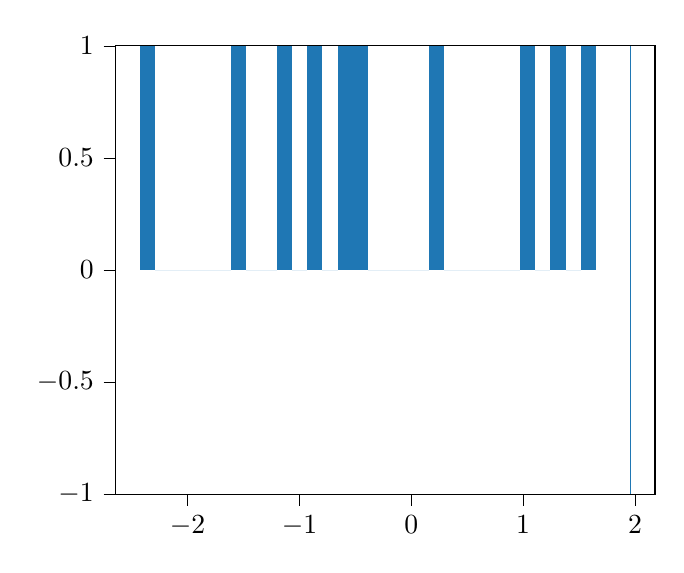
\begin{tikzpicture}

\definecolor{darkgray176}{RGB}{176,176,176}
\definecolor{steelblue31119180}{RGB}{31,119,180}

\begin{axis}[
tick align=outside,
tick pos=left,
x grid style={darkgray176},
xmin=-2.6460132, xmax=2.179334,
xtick style={color=black},
y grid style={darkgray176},
ymin=-1, ymax=1,
ytick style={color=black}
]
\draw[draw=none,fill=steelblue31119180] (axis cs:-2.4266792,0) rectangle (axis cs:-2.2907421,1);
\draw[draw=none,fill=steelblue31119180] (axis cs:-2.2907421,0) rectangle (axis cs:-2.1548049,0);
\draw[draw=none,fill=steelblue31119180] (axis cs:-2.1548049,0) rectangle (axis cs:-2.0188677,0);
\draw[draw=none,fill=steelblue31119180] (axis cs:-2.0188677,0) rectangle (axis cs:-1.8829305,0);
\draw[draw=none,fill=steelblue31119180] (axis cs:-1.8829305,0) rectangle (axis cs:-1.7469933,0);
\draw[draw=none,fill=steelblue31119180] (axis cs:-1.7469933,0) rectangle (axis cs:-1.6110561,0);
\draw[draw=none,fill=steelblue31119180] (axis cs:-1.6110561,0) rectangle (axis cs:-1.4751189,1);
\draw[draw=none,fill=steelblue31119180] (axis cs:-1.4751189,0) rectangle (axis cs:-1.3391817,0);
\draw[draw=none,fill=steelblue31119180] (axis cs:-1.3391817,0) rectangle (axis cs:-1.2032445,0);
\draw[draw=none,fill=steelblue31119180] (axis cs:-1.2032445,0) rectangle (axis cs:-1.0673073,1);
\draw[draw=none,fill=steelblue31119180] (axis cs:-1.0673073,0) rectangle (axis cs:-0.93137012,0);
\draw[draw=none,fill=steelblue31119180] (axis cs:-0.93137012,0) rectangle (axis cs:-0.79543293,1);
\draw[draw=none,fill=steelblue31119180] (axis cs:-0.79543293,0) rectangle (axis cs:-0.65949574,0);
\draw[draw=none,fill=steelblue31119180] (axis cs:-0.65949574,0) rectangle (axis cs:-0.52355855,1);
\draw[draw=none,fill=steelblue31119180] (axis cs:-0.52355855,0) rectangle (axis cs:-0.38762135,1);
\draw[draw=none,fill=steelblue31119180] (axis cs:-0.38762135,0) rectangle (axis cs:-0.25168416,0);
\draw[draw=none,fill=steelblue31119180] (axis cs:-0.25168416,0) rectangle (axis cs:-0.11574697,0);
\draw[draw=none,fill=steelblue31119180] (axis cs:-0.11574697,0) rectangle (axis cs:0.020190225,0);
\draw[draw=none,fill=steelblue31119180] (axis cs:0.020190225,0) rectangle (axis cs:0.15612742,0);
\draw[draw=none,fill=steelblue31119180] (axis cs:0.15612742,0) rectangle (axis cs:0.29206461,1);
\draw[draw=none,fill=steelblue31119180] (axis cs:0.29206461,0) rectangle (axis cs:0.4280018,0);
\draw[draw=none,fill=steelblue31119180] (axis cs:0.4280018,0) rectangle (axis cs:0.563939,0);
\draw[draw=none,fill=steelblue31119180] (axis cs:0.563939,0) rectangle (axis cs:0.69987619,0);
\draw[draw=none,fill=steelblue31119180] (axis cs:0.69987619,0) rectangle (axis cs:0.83581338,0);
\draw[draw=none,fill=steelblue31119180] (axis cs:0.83581338,0) rectangle (axis cs:0.97175057,0);
\draw[draw=none,fill=steelblue31119180] (axis cs:0.97175057,0) rectangle (axis cs:1.1076878,1);
\draw[draw=none,fill=steelblue31119180] (axis cs:1.1076878,0) rectangle (axis cs:1.243625,0);
\draw[draw=none,fill=steelblue31119180] (axis cs:1.243625,0) rectangle (axis cs:1.3795622,1);
\draw[draw=none,fill=steelblue31119180] (axis cs:1.3795622,0) rectangle (axis cs:1.5154993,0);
\draw[draw=none,fill=steelblue31119180] (axis cs:1.5154993,0) rectangle (axis cs:1.6514365,1);
\addplot [semithick, steelblue31119180]
table {%
1.96 -1
1.96 1
};
\end{axis}

\end{tikzpicture}
